\chapter{Programación PLC}
\label{ch:progPLC}

Uno de las partes principales de este trabajo es la programación del \gls{plc}. 
Una vez montado todo el sistema, 
realizado el cableado eléctrico y verificado su correcto funcionamiento
para verificar la seguridad del sistema se procedió a la programación.

En el presente capítulo se describe tanto el algoritmo del programa que se grabo
en el \gls{plc}, así como el 
lenguaje utilizado y las diferentes herramientas que ofrece el software 
con el que se trabajo para poder llevar a cabo la tarea.

\section{Algoritmo}
\label{sec:Algoritmo}
Para comenzar la programación realizada en el lenguaje ladder,
se pensó en el algoritmo que nos permitiría realizar las acciones
necesarias para alcanzar los objetivos propuestos. Comenzamos describiendo
en el algoritmo \ref{img:algoritmo} como de manera estructurada nuestro
sistema debe comportarse.

\begin{algorithm}[H]

 \While{el tablero este energizado}{
  señal de PLC run\;
  adquisición de nivel, caudal y Set Point\;
  
  \eIf{nivel > HHL}{
   alerta de HHL y detención del sistema\;
   }{}
  \eIf{nivel < LLL}{
    alerta LLL y detención del sistema\;}{}
  
  \eIf{nivel > HL}{
   alerta de HL\;}{
   limpieza de alerta\;}
  
  \eIf{nivel < LL}{
    alerta LL\;}{
    limpieza de alerta\;}
  
  \eIf{deseo setear parámetros del controlador}{
    adquisición Kp, Ti y Td\;}{}
    
  \eIf{deseo controlar el sistema manualmente}{
    
    \eIf{motor 1}{activo motor 1\;}{}
    \eIf{motor 2}{activo motor 2\;}{}
    \eIf{válvula}{activo bandera para el bloque del controlador PID}{}
    }{
    el sistema continúa trabajando en modo automático\;
    }
  bloque del controlador PID\;
  constatar que el sistema funciona segun lo esperado\;
  }
  
 \caption{Algoritmo de programación}
 \label{img:algoritmo}
\end{algorithm}

\section{Programación}
\label{sec:Programacion}
Se utilizó el programa Twido Soft para poder programar el \gls{plc}. Se programó
en lenguaje Ladder.

El lenguaje Ladder es muy común en la programación de automatas debido a que es un 
lenguaje gráfico que esta basado en esquemas eléctricos de control clásicos. En el
de acuerdo a una combinación de contactos en la entrada se obtiene una acción en la
salida. De esta manera paso a paso vamos describiendo las acciones que deseamos
realice el controlador de acuerdo al estado del sistema o las ordenes recibidas desde
el escada.

Entre otros, los elementos de entrada con los que cuenta el programa son:

 \begin{itemize}
  \item Contacto normalmente abierto
  \item Contacto normalmente cerrado
 \end{itemize}
 
Como acciones de salida encontramos la siguientes:

  \begin{itemize}
   \item Tomar el valor lógico de la función de entrada.
   \item Tomar el valor lógico negado de la función de entrada.
   \item Seteo la bobina de salida.
   \item Reseteo de la bobina de salida.
  \end{itemize}

El software Twido Soft sirve tanto como para enviar el programa al \gls{plc}, así como 
para descargar el programa que esta en el \gls{plc}. A tal efecto a continuación 
se explicaran algunas cualidades del programa para que sea simple su comprensión.

Lo primero que se presenta son la acción realizada en cada RUNG (pasos del programa).


\begin{tikzpicture}[
  grow via three points={one child at (0.5,-0.7) and
  two children at (0.5,-0.7) and (0.5,-1.4)},   
  edge from parent path={(\tikzparentnode.south) |- (\tikzchildnode.west)}]
  \node (init) {Inicio del programa  }
    child { node {Inicialización} }
    child { node {Señal PLC run}    }
    child { node {Adquisición de Nivel y Caudal}    }
    child { node {Gestión de alarmas HHL y LLL}    }
    child { node {Gestión de banderas de alarmas HHL y LLL}    }
    child { node {Seteo de parámetros del controlador: Kp}    }
    child { node {Seteo de parámetros del controlador: Ti}    }
    child { node {Seteo de parámetros del controlador: Td}    }
    child { node {Seteo de parámetros del controlador: Set Point}    }
    child { node {Gestión de bandera de encendido y parada del sistema}    }
    child { node {Gestión de bandera de modo manual y automático}    }
    child { node {Gestión de motores si el sistema esta en modo automático}    }
    child { node {Encendido del Motor 1: Control manual y automático}    }
    child { node {Encendido del Motor 2: Control manual y automático}    }
    child { node {Controlador: PID}    }
    child { node {Valor de salida de la válvula}    }
    child { node {Gestión de señal indicadora del estado del sistema: manual o automático}    }
    child { node {Indicador del estado del Motor 1}    }
    child { node {Indicador del estado del Motor 2}    }
    child { node {Indicador de error en bombas}    }
    child { node {Gestión de bandera del sistema trabajando en modo normal}    }
    child { node {Limpieza de alarmas}    };
  
\end{tikzpicture}
\tikzstyle{every node}=[] % resets borders of tables
\tikzstyle{selected}=[] % resets selected

\todo{Anexo de lo que imprimimos desde el twido soft}


El programa presenta baderas que nos sirven para conocer diferentes estados
de la planta. En la tabla \ref{table:Banderasinternas} se pueden ver el nombre 
de las mismas y sus funciones.


\begin{table}[!t]

\renewcommand{\arraystretch}{1.3}
\centering
\begin{tabular}{c||c}
\hline
\bfseries Memoria & \bfseries Descripción\\
\hline \hline
\verb|M0|  & Bandera de inicialización\\
\verb|M1|  & Sistema Encendido/Apagado\\
\verb|M2|  & Sistema en modo Manual/Automático\\
\verb|M3|  & Error de Nivel\\
\verb|M4|  & Error de Motor\\
\hline
\end{tabular}
\caption{Banderas internas}
\label{table:Banderasinternas}
\end{table}

Por ultimo se expresan las entradas y salidas al \gls{plc}, tanto analógicas
como discretas en la tabla \ref{table:entradassalidas}.

\begin{table}[!t]

\renewcommand{\arraystretch}{1.3}
\centering
\begin{tabular}{c||c}
\hline
\bfseries Memoria & \bfseries Descripción\\
\hline \hline
\verb|Q0.0|  & Encender motor 1\\
\verb|Q0.1|  & Encender motor 2\\
\verb|Q0.7|  & Señal de encendido de los motores\\
\verb|I0.0|  & Retroalimentación desde el relevo térmico motor 1\\
\verb|I0.1|  & Retroalimentación desde el relevo térmico motor 2\\
\verb|IW0.1.0|  & Señal analógica de nivel\\
\verb|IW0.1.1|  & Señal analógica de caudal \\
\verb|QW0.1.0|  & Señal analógica de salida de apertura de la válvula \\
\hline
\end{tabular}
\caption{Entradas y salidas al PLC}
\label{table:entradassalidas}
\end{table}

\section{Comunicación}
\label{sec:Comunicacion}

Para ser capaces de interactuar con la aplicación de \gls{scada} definimos
ciertas palabras que nos permiten realizar acciones en el sistema y conocer
el estado del mismo.

La tabla \ref{table:bitlecturasescrituras} presenta dos palabras de dieciséis
bits, \verb|MW0| y \verb|MW1|, la primera de ella presenta bits de lectura, en donde se
refleja el estado del la plata, mientras que la segunda palabra sus bits son
de escritura y nos da la posibilidad de manejar la planta.
\begin{table}[!t]

\renewcommand{\arraystretch}{1.3}
\centering
\begin{tabular}{c||c||c||c}
\hline
\bfseries Tipo & \bfseries Word & \bfseries Bit & \bfseries Descripción\\
\hline \hline
Lect & \verb|MW0| & \verb|X0| & Señal Run PLC\\
Lect & & \verb|X1| & Alarma HHL\\
Lect & & \verb|X2|& Alarma LLL\\
Lect & & \verb|X3|& Alarma HL\\
Lect & & \verb|X4|& Alarma LL\\
Lect & & \verb|X5|& Error en motores (era \verb|MW0:X13|)\\
Lect & & \verb|X6|& Motor 1 encendido (era \verb|MW0:X11|)\\
Lect & & \verb|X7|& Motor 2 encendido(era \verb|MW0:X12|)\\
Lect & & \verb|X8|& Modo manual activado (era \verb|MW0:X14|)\\
Lect & & \verb|X9|& Modo automático activado y funcionando (Nuevo)\\
Lect & & \verb|X10|& Planta funcionando sin errores (era \verb|MW0:X15|)\\
\hline
Esc & \verb|MW1| & \verb|X0|& Switch modo manual/automático (era 
\verb|MW0:X10|)\\
Esc & & \verb|X1|& Aplicar (era \verb|MW0:X15|)\\
Esc & & \verb|X2|& Encender/Apagar (automático) (era \verb|MW0:X9|)\\
Esc & & \verb|X3|& Se desea cambiar el PID (era \verb|MW0:X6|)\\
Esc & & \verb|X4|& Se desean los valores por default para el PID (era 
\verb|MW0:X7|)\\
Esc & & \verb|X5|& Se desean valores por default para SP (era \verb|MW0:X8|)\\
Esc & & \verb|X6|& Encender M1 (manual) (era \verb|MW8:X1|)\\
Esc & & \verb|X7|& Encender M2 (manual) (era \verb|MW8:X2|)\\
Esc & & \verb|X8|& Limpiar errores (era \verb|MW8:X0|)\\
\hline

\hline
\end{tabular}
\caption{Bits lectura/escritura}
\label{table:bitlecturasescrituras}
\end{table}

Por otro lado la tabla \ref{table:palabraslecturasescrituras} nos presenta 
las palabras de las restantes palabras de memoria que ocupa el programa, en 
la primer parte de la tabla se encuentran las palabras de solo lectura que 
presentan los valores que presentan las variables del sistema, mientras que en la 
segunda parte de la misma se encuentran las memorias reservadas al cambio
de los parámetros del sistema.

\begin{table}[!t]

\renewcommand{\arraystretch}{1.3}
\centering
\begin{tabular}{c||c||c}
\hline
\bfseries Tipo & \bfseries Word  & \bfseries Descripción\\
\hline \hline
Lect & \verb|MW2|  & Lectura DP cell nivel (era \verb|MW1|)\\
Lect & \verb|MW3|  & Lectura DP cell caudal\\
Lect & \verb|MW4|  & Valor Kp\\
Lect & \verb|MW5|  & Valor Ki\\
Lect & \verb|MW6|  & Valor Kd\\
Lect & \verb|MW7|  & Valor de lectura del SP (era \verb|MW2|)\\
Lect & \verb|MW8|  & Valor de lectura de la válvula (era \verb|MW7|)\\
\hline
Esc & \verb|MW9| & Valor de escritura de la válvula (manual) (era 
\verb|MW15|) \\
Esc & \verb|MW10|  & Valor de escritura del SP \\
Esc & \verb|MW11|  & Valor de escritura Kp \\
Esc & \verb|MW12|  & Valor de escritura Ki \\
Esc & \verb|MW13| & Valor de escritura Kd \\
\hline
\end{tabular}
\caption{Palabras lectura/escritura}
\label{table:palabraslecturasescrituras}
\end{table}

\section{Controlador PID}
\label{sec:controladorpid}

En un controlador \gls{pid} la acción correctiva se toma de manera que:

\begin{itemize}
 \item Proporcional al error.
 \item Proporcional a la integral del error respecto del tiempo
 \item Proporcional a la derivada del error respecto del tiempo
\end{itemize}

El software Twido Soft ofrece un modulo \gls{pid} que nos ofrece las
opciones que necesitamos.

\begin{itemize}
 \item Módulo automático: se le debe suministrar el valor de las ganancias. 
 \item Opción de apertura manual.
\end{itemize}

En la tabla \ref{table:controladorpid} se muestra la configuración del 
controlador PID.

\begin{table}[!t]

\renewcommand{\arraystretch}{1.3}
\centering
\begin{tabular}{c||c||c}
\hline
\bfseries Tipo & \bfseries Word  & \bfseries Descripción\\
\hline \hline
Entrada & \verb|IW1.0|  & Medida\\
\hline
PID & \verb|MW2|  & Consigna\\
PID & \verb|Kp|  & Ganancia proporcional\\
PID & \verb|Ti|  & Ganancia integral\\
PID & \verb|Td|  & Ganancia derivativa\\
\hline
Salida & \verb|M2|  & Modo manual\\
Salida & \verb|MW15|  & Salida\\
Salida & \verb|QW1.0|  & Salida digital\\
\hline
\end{tabular}
\caption{Entradas y salidas al PID}
\label{table:controladorpid}
\end{table}

Para accionar la válvula de manera manual el bloque tiene una bandera
que una vez activada permite que la salida del módulo, siendo esta la 
apertura de la válvula, sea una palabra de memoria. De esta manera se 
permite el control control de la válvula desde el software \gls{scada}.

\subsection{Determinación de las ganancias}

Para poder determinar las ganancias del controlador se decidió seguir
las reglas propuestas por ZIEGLER–NICHOLS, las cuales analizán la respuesta
del sistema a una perturbación en escalón.

Se presentan dos métodos:
\begin{itemize}
 \item Primer método:
 
 Se obtiene experimentalmente la respuesta de la planta a una entrada en escalón,
 si la respuesta es similar a la de la imagen \ref{fig:primermetodo}.
 La respuesta puede ser caracterizada por dos constantes, el tiempo de delay L y una
 constante de tiempo T. Estas pueden ser halladas dibujando una recta tangente al 
 punto de inflexión de la curva de la respuesta del sistema, a partir la intersección de
 esta recta con el eje del tiempo como muestra la figura \ref{fig:primermetodo}.
 
 \item Segundo método:
 
 Este método comienza su análisis con un controlador puramente proporcional. Se incrementa 
 la ganancia proporcional desde cero hasta un valor $Kp_{cr} $ donde la respuesta del 
 sistema presenta oscilaciones como en la imagen \ref{fig:segundometodo}.
 A partir de esto hemos obtenido experimentalmente $Kp_{cr} $ y $P_{cr} $.
\end{itemize}


\begin{figure}
 \centering
 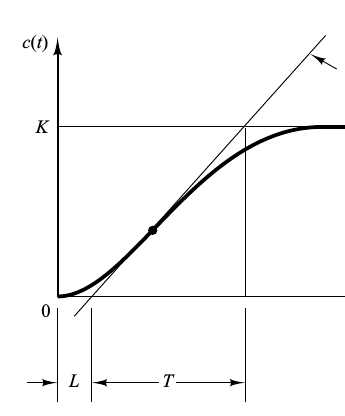
\includegraphics[scale=0.5]{Cap4-ProgramacionPLC/images/primermetodo.png}
 \caption{Respuesta del sistema a un escalón.}
 \label{fig:primermetodo}
\end{figure}


\begin{figure}
 \centering
 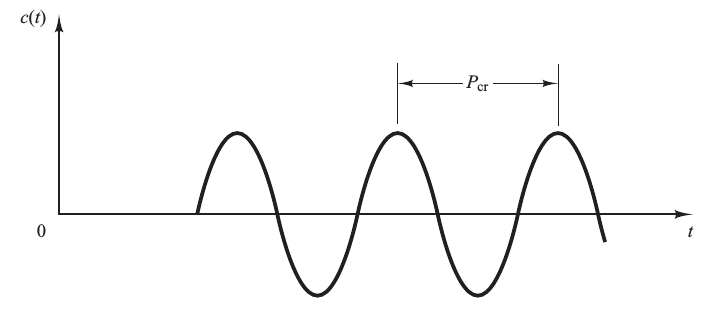
\includegraphics[scale=0.5]{Cap4-ProgramacionPLC/images/segundometodo.png}
 \caption{Oscilacion sostenida del sistema.}
 \label{fig:segundometodo}
\end{figure}

A partir de los datos obtenidos con la respueta experimental del sistema
ZIEGLER–NICHOLS proponen elegir el valor de las ganancias de acurdo a los
valores de la tabla \ref{table:valorganancias}.


\begin{table}[!t]

\renewcommand{\arraystretch}{1.3}
\centering
\begin{tabular}{c||c||c |c}
\hline
\bfseries Método & \bfseries Kp  & \bfseries Ti & \bfseries Td\\
\hline \hline
Primero &  $ 1.2 \, \dfrac{T}{L}$ & $2 \, L $ & $ 0.5 \, L $\\
\hline
Segundo &  $0.6 \,Kp_{cr}  $ & $ 0.5 \, P_{cr}$ & $0.125 \, P_{cr} $\\
\hline
\end{tabular}
\caption{Valor de las ganacias}
\label{table:valorganancias}
\end{table}


\section{Depuración (Debug)}
\label{sec:Debug}


Una vez finalizada la programación y antes de unirlo al software \gls{scada} 
se realizaron las pruebas correspondientes al correcto funcionamiento y respuesta
a las situaciones posibles. 

El software Twido Soft presenta una animación que nos permite realizar un debug en
tiempo de funcionamiento, sabiendo así la situación real del sistema. 
La animación colorea las bobinas que están activas de acuerdo a lo especificado
en las líneas del programa.

También podemos forzar el estado de algunas bobinas y cambiar el valor de las 
palabras de memoria. Esto nos permite generar las situaciones deseadas.
Fue muy importante tener esta herramienta para poder analizar el código propuesto
dada su practicidad, y poder realizar los cambios necesarios.

Las pruebas realizadas fueron las siguientes:

\begin{itemize}
 \item Lectura de las variables.
 
 Al tener acceso a todas las palabras de memoria se tuvo la precaución de mantener el
 sistema apagado y se constato que los valores recogidos desde la entrada analógica
 tengan sentido con lo que sucede en el sistema. Para ello el caudal debía ser cero debido
 a que no estaba circulando fluido y la altura debía coincidir con lo mostrado por el 
 indicador visual de nivel. 
 
 \item Correcto funcionamiento del Controlador y adquisición del Set Point.
 
 Se le dio al sistema un Set Point y se verificó su correcto funcionamiento. 
 La característica principal de esta prueba fue que estaban deshabilitadas las demás
 funciones del sistema, solo interesaba saber como respondía el bloque controlador.
 El primer valor otorgado fue al 50 porciento, luego se hizo variar al 25 porciento
 y por ultimo al 75 porciento.
 
 \item Correcto funcionamiento de las alarmas y paradas de emergencia.
 
 Para poder detectar esta situaciones del sistema se forzo un estado que no es el normal
 de funcionamiento, se forzo a desplazar el sistema por encima y por debajo de los
 límites de funcionamiento para conocer la respuesta del sistema. Lo que se esperaba en esta
 prueba era ver el cambio en la palabra que contiene el estado del sistema.
 
 Para las alarmas de Low Level y High Level solo se envía una señal al software \gls{scada},
 se verifico correctamente el cambio en la palabra \verb|MW0|.
 
 Para las alarmas de Low Low Level y High High Level, no solo se constato el cambio en la
 palabra \verb|MW0|, que representa el cambio en el estado de la planta sino que además 
 se procede a la detención de la planta.
 
 Estas pruebas fueron muy importantes dado que se hizo trabajar al sistema en una situación
 crítica.
 
 \item Encendido y parada del sistema en modo manual.
 
 Para poder inferir sobre el sistema se debe cambiar la palabra \verb|MW1|, se procedio a
 hacer funcionar al sistema de modo automático, con un nivel de Set Point preestablecido.
 
 \item Seteo de parámetros.
 
 Hasta este momento los valores de las ganancias del controlador eran las establecidas por 
 default, una vez asegurados que funcionaba el sistema y sobre todo las paradas de emergencias
 se probó el seteo de parámetros, modificando la palabra \verb|MW1| y la correspondiente 
 memoria de acuerdo al valor que se desee modificar.
 
 \item Control del sistema en modo manual.
 
 Otra vez modificando la palabra \verb|MW1| se eligió manejar el sistema de modo manual.
 Una vez el sistema en modo manual se debe mandar el valor de apertura de la válvula y 
 la señal para encender cada motor por separado
 
 \item Retroalimentación del estado del sistema.
 
 En esta prueba solo se constato que los valores de las palabras de memoria sean lógicos,
 se hicieron pruebas de todas las situaciones anteriores con las paradas de emergencia 
 habilitadas.
 
 \item Parada de emergencia por error en el funcionamiento de los motores.
 
 Por ultimo se forzó nuevamente al sistema a una situación extrema, en la que uno
 de los motores se para por sobrecalentamiento por ejemplo. Lo que esperamos es que se
 detenga el sistema una vez que forcemos una salida y la retroalimentación que indica que
 ese motor se encendió no se active.
 
\end{itemize}

En la imagen \ref{img:twidosoftdebug} se puede apreciar las table que nos permite realizar
el debug desde el programa.

\begin{figure}[ht!]
	\centering
	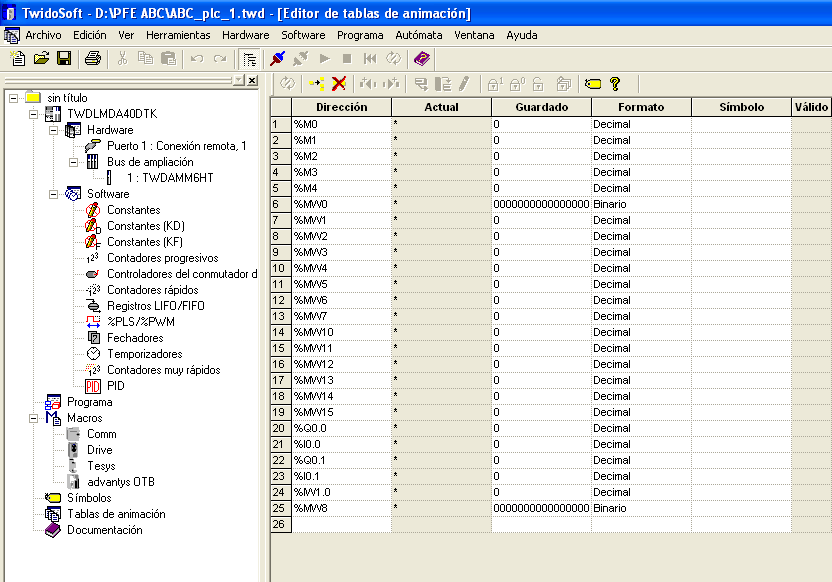
\includegraphics[scale=0.5]{Cap4-ProgramacionPLC/images/twidosoftdebug.png}
	\caption{Esquema de la división del tiempo}
	\label{img:twidosoftdebug}
\end{figure}